\FloatBarrier
\section{Combined Dynamics} \label{sec:combined}

It is possible to define a set of dynamics to run a combination of the dynamics. 
The resulting dynamic is defined as 
\begin{equation}
\dot{ x } = \sum_{d\in \mathcal{D}} \gamma_d V_d( x ),
\end{equation}
where $\mathcal{D}=\{ Logit, RD, Smith, BNN \}$ denotes the set of available dynamics, $V_d()$ is the differential equation of the $d\th$ dynamic and $\gamma_d$ is the weight assigned to it.
The dynamics should be defined in a cell array, e.g., 
\begin{lstlisting}
dynamics = {'bnn', 'rd'};
\end{lstlisting}
The combination is made making a linear combination between each dynamic listed in the cell array. The weight assigned to each dynamic is defined in the vector \verb|gamma|. In this case we assign 
\begin{lstlisting}
gamma = [.25, .75]; 
\end{lstlisting}

Fig. \ref{fig:rps_combined} shows an example of the combined dynamics for the rock-paper-scissors game. Note that the evolution of the system is not confined to a limit cycle, as happened with the replicator dynamics in Fig.  \ref{fig:finite1}.

\begin{figure}[h]
  \centering
  \begin{subfigure}[b]{0.4\textwidth}
	  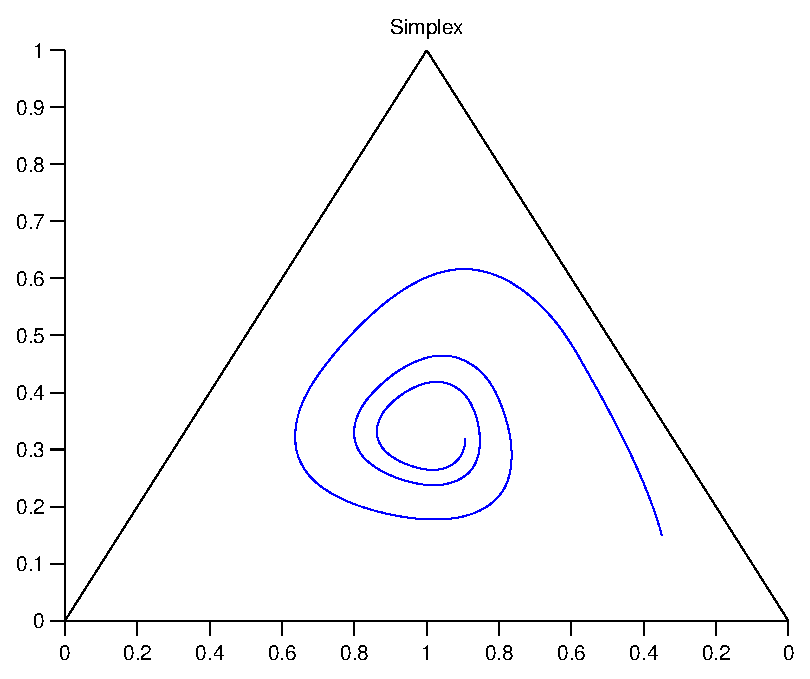
\includegraphics[width=\textwidth]{./images/test_combined.eps}
	  \caption{Simplex.}
	  \label{fig:test_combined_simplex}
  \end{subfigure}
  ~ 
  \begin{subfigure}[b]{0.45\textwidth}
	  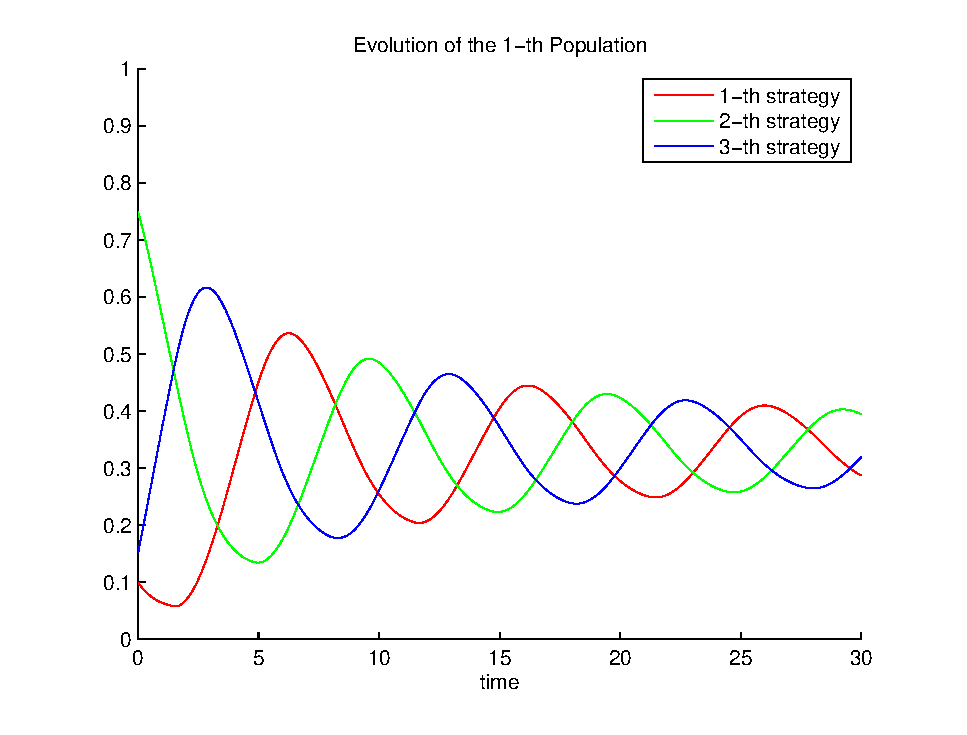
\includegraphics[width=\textwidth]{./images/test_combined_ev.eps}
	  \caption{Evolution of the strategies in time.}
	  \label{fig:test_combined_ev}
  \end{subfigure}
  \caption{Evolution of the combination of replicator dynamics and BNN dynamics.}
  \label{fig:rps_combined}
\end{figure}



